\documentclass[UTF8, a4paper]{ctexart}
\usepackage[margin=1in]{geometry} % 页边距调整
\usepackage{ctex}
\usepackage{array, amsmath, amssymb}

\usepackage{booktabs, tabularx, multirow, multicol} % 表格拓展支持
\usepackage{graphicx, subfigure, float} % 图片排版支持

\usepackage{algorithm, algpseudocode} % 伪代码支持
\renewcommand{\algorithmicrequire}{\textbf{Input:}}  
\renewcommand{\algorithmicensure}{\textbf{Output:}} 

\usepackage{tikz, mathpazo} % 基本绘图支持
\usepackage{flowchart} % 流程图支持
\usepackage{pgf-umlcd} % UML类图支持
\usetikzlibrary{arrows, shapes, chains, shapes.geometric}

\usepackage{listings} % 代码块支持
\usepackage{xcolor}
\lstset{
	language		= c++,
	backgroundcolor	= \color{white},
	basicstyle		= \footnotesize\ttfamily,
	keywordstyle	= \color{blue},
	stringstyle		= \color{red!58!blue!82}\ttfamily,
	commentstyle	= \color{darkgray},
	rulesepcolor	= \color{red!20!green!20!blue!20},
	columns			= fullflexible,
	breaklines		= true,
	captionpos		= b,
	tabsize			= 4,
	frame			= single,
	escapeinside	= {\%*}{*)}
}
%%示例
% \begin{lstlisting}[caption={}]
% #include <iostream>
% int main(int argc, char *argv[]) {
% 	std::cout << "Hello World!" << std::endl;
% 	return 0;
% }
% \end{lstlisting}

\usepackage{datetime} %日期
\renewcommand{\today}{\number\year{年}\number\month{月}\number\day{日}}

\begin{document}

\begin{center}
	\zihao{3}《数据结构》实验报告
\end{center}
\zihao{5}

\newcolumntype{Y}{>{\raggedleft\arraybackslash}X}
\noindent\begin{tabularx}{\textwidth}{XcY}
	  {班 级:}\;\underline{DL062123}
	& {姓 名:}\;\underline{项乔栋}
	& {学 号:}\;\underline{2021302468} \\
	  {邮 箱:}\;\underline{13282135976@sina.cn}
	& {日 期:}\;\underline{\today}
	& {编 号:}\;\underline{DS04}
\end{tabularx}
~\\

\noindent\textbf{$\circledcirc$
实验题目:\quad{稀疏矩阵相加}} \par
\noindent\textbf{$\circledcirc$
实验目的:\quad{实践密集矩阵方法到稀疏矩阵的迁移}} \par
\noindent\textbf{$\circledcirc$
实验内容:\quad{基于三元组的稀疏矩阵加法实现}} \par

\subsection*{一、需求分析}
\noindent\fbox{
\begin{tabularx}{\textwidth}{lY}
\bf{Description}
& \parbox[t]{\linewidth}{
	输入两个稀疏矩阵,输出它们相加的结果。
} \\

\bf{Input}
& \parbox[t]{\linewidth}{
	第一行输入四个正整数,分别是两个矩阵的行m、列n、第一个矩阵的非零元素的个数t1和第二个矩阵的非零元素的个数t2。接下来的t1+t2行是三元组,分别是第一个矩阵的数据和第二个矩车的数据。三元组的第一个元素表示行号,第二个元素表示列号,第三个元素是该项的值。
} \\

\bf{Output}
& \parbox[t]{\linewidth}{
	输出相加后的矩阵三元组
} \\

\bf{Sample Input}
& \fbox{\parbox[t]{\linewidth}{\bf{
	\mbox{3 4 3 2} \\
	\mbox{1 1 1} \\
	\mbox{1 3 1} \\
	\mbox{2 2 2} \\
	\mbox{1 2 1} \\
	\mbox{2 2 3}
}}} \\

\bf{Sample Output}
& \fbox{\parbox[t]{\linewidth}{\bf{
	\mbox{1 1 1} \\
	\mbox{1 2 1} \\
	\mbox{1 3 1} \\
	\mbox{2 3 5}
}}}
\end{tabularx}}

\subsection*{二、概要设计}
为保持基于三元组的稀疏矩阵的有序性并兼顾算法效率,使用统计方法预处理稀疏矩阵,得到相关信息,以直接定位转置后元素的位置。 \par
1.\;基本操作: \par
	CreateFromIO() $\rightarrow$ SparseMatrix \par
	\qquad\textbf{操作结果:}\;从IO流创建稀疏矩阵 \par
	Add(lhs:SparseMatrix,rhs:SparseMatrix) $\rightarrow$ SparseMatrix \par
	\qquad\textbf{操作结果:}\;获取稀疏矩阵的加和 \par
	Output(matrix:SparseMatrix) $\rightarrow$ void \par
	\qquad\textbf{操作结果:}\;输出稀疏矩阵 \par
2.\;程序模块: \par
1) 主程序 \par
2) IO支持 \par
3) 稀疏矩阵加法 \par
\begin{figure}[H]
	\begin{minipage}[t]{\linewidth}
		\centering
		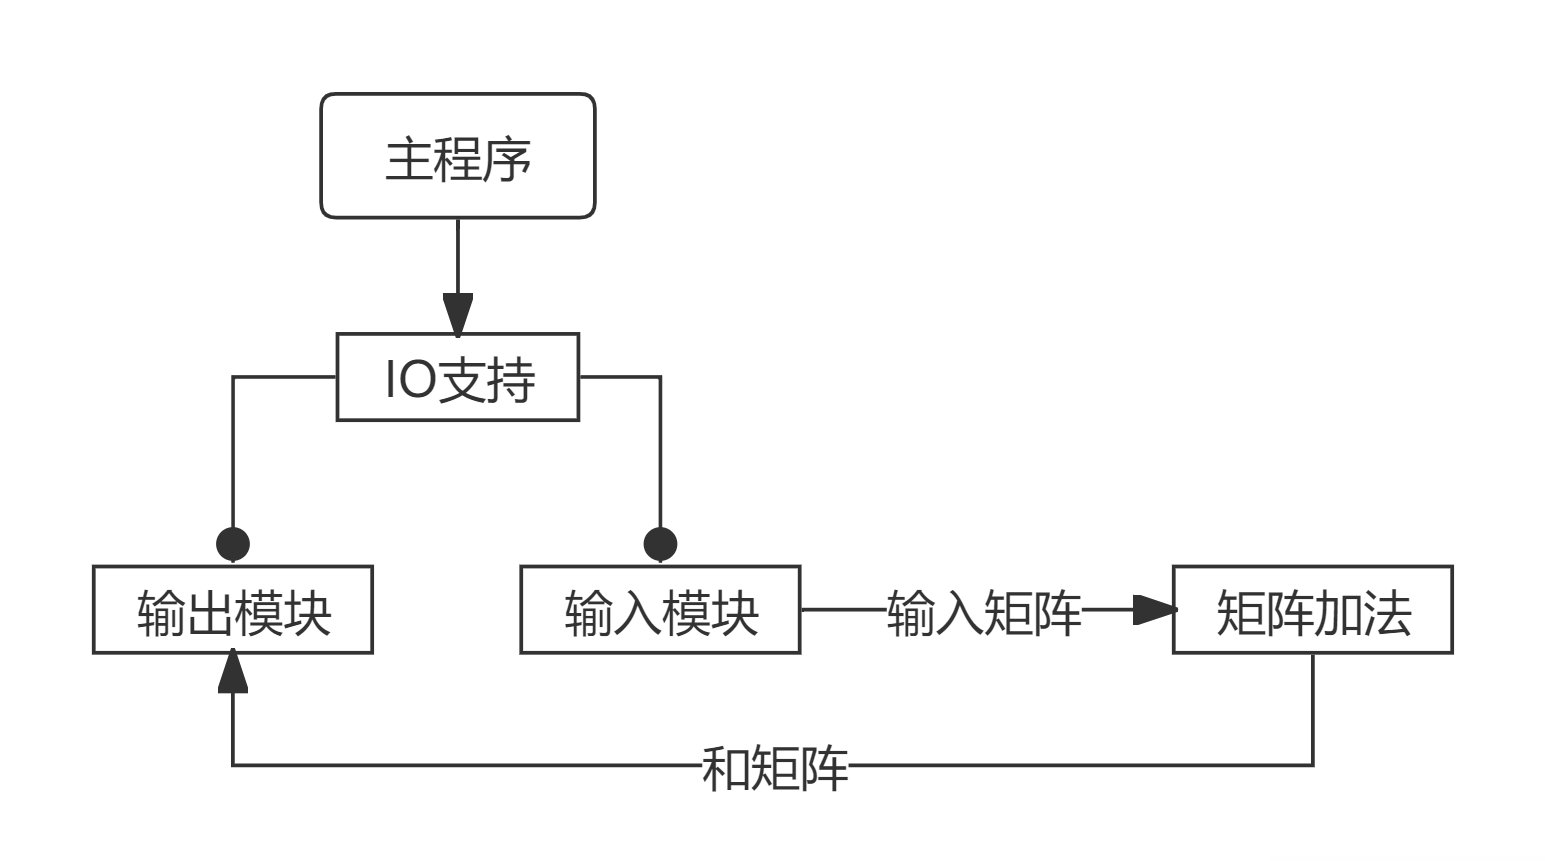
\includegraphics[width=125mm,height=64mm]{./assets/DS04-1}
	\end{minipage}
\end{figure}

\subsection*{三、详细设计}
\begin{algorithm}
\begin{algorithmic}[1]
\caption{Sparse Matrix Addition based on Triple}
\Require SparseMatrix: $\mathbf{A}$,$\mathbf{B}$
\Ensure A+B as SparseMatrix
\State let $\mathbf{C}$ $\leftarrow$ SparseMatrix
\While {$\mathbf{A}\neq\emptyset$ and $\mathbf{B}\neq\emptyset$}
	\State let $\mathbf{a}$ $\leftarrow$ next triple in $\mathbf{A}$
	\State let $\mathbf{b}$ $\leftarrow$ next triple in $\mathbf{B}$
	\If {$\mathbf{a}$ and $\mathbf{b}$ are in the same position}
		\If {$(\mathbf{a}+\mathbf{b}).value\neq 0$}
			\State append $\mathbf{a}+\mathbf{b}$ to $\mathbf{C}$
		\EndIf
		\State remove $\mathbf{a},\mathbf{b}$ from $\mathbf{A},\mathbf{B}$
	\Else
		\State select the small-order one in $\mathbf{a},\mathbf{b}$ as $\mathbf{it}$
		\State append $\mathbf{it}$ to $\mathbf{C}$
		\State remove $\mathbf{it}$ from relevant matrix
	\EndIf
\EndWhile
\State return $\mathbf{C}$
\end{algorithmic}
\end{algorithm}

\subsection*{四、使用说明、测试分析与结果}
\subsubsection*{1、使用说明}
1) 本程序可以通过任意编译器生成目标文件并在当前平台运行。 \par
2) 进入程序后依照需求的输入样式输入数据,手动输入与流式输入都是被允许的。特别的是,你应当保证输入的数组长度不大于100。 \par
\subsubsection*{2、测试结果与分析}
2.1\;\textbf{实际环境} \par
对于所有输入,矩阵元素以行主序输入\par
2.2\;\textbf{边界情况} \par
矩阵和产生零值元素 \par
2.3\;\textbf{测试结果} \par
目标代码通过全部测试,无需纠正
\subsubsection*{3、调试过程问题分析与解决办法}
编码与测试环节皆未产生问题,跳过调试环节
\subsubsection*{4、设计与实现的回顾讨论与分析}
三元组稀疏矩阵之和,首先考虑该类矩阵本身的性质。其一是有序性,其二是不存在非零元素。那么在求和时只需保证从两个操作数矩阵按顺序插入三元组,并舍弃加和为零的元素,就完成了算法的整个流程。
\subsubsection*{5、运行界面}
\begin{figure}[H]
	\begin{minipage}[t]{\linewidth}
		\centering
		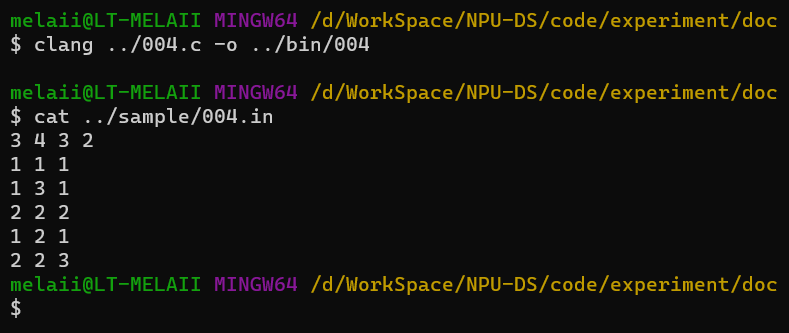
\includegraphics[width=125mm,height=50mm]{./assets/DS04-2}
		\caption{前置环境}
	\end{minipage}
\end{figure}
\begin{figure}[H]
	\begin{minipage}[t]{\linewidth}
		\centering
		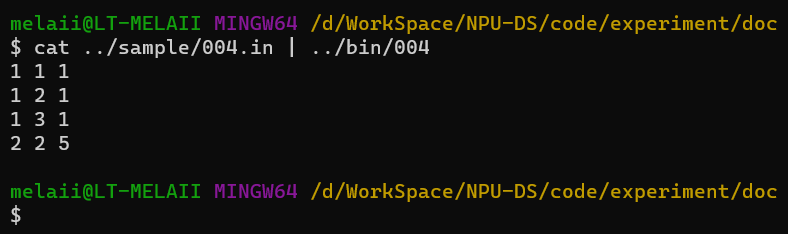
\includegraphics[width=125mm,height=40mm]{./assets/DS04-3}
		\caption{结果输出}
	\end{minipage}
\end{figure}

\subsection*{五、实验总结}
三元组稀疏矩阵求和,可以说归为有序序列的合并。唯一多出的地方就是相同的值需要被加和,而加和值为零的元素需要被舍弃。如此思考,其实该和也不是什么特别地东西,无非就是基础问题加了点边角料。进一步思考,稀疏矩阵之和直觉上将会使该矩阵产生更多的元素,而当加和次数足够多时,该矩阵将不再稀疏,稀疏矩阵存储方法也失去了意义,变得比常规存储更加耗时、复杂。在实际应用上,当发觉稀疏矩阵元素数目超过某一个阈值时将其转换为常规存储形式,这或许是个不错的想法。

~\\
\zihao{-4}
\textbf{教师评语:}
~\\
\textbf{实验成绩:}

\begin{flushright}
\mbox{指导教师签名:\qquad\qquad} \\
\mbox{批阅日期:\qquad\qquad}
\end{flushright}

\end{document}